\subsection{Geometrical Reconstruction}
\label{sec:gr}

The geometrical reconstruction is based on the \babar DIRC approach~\cite{bdirc1}. This approach transforms the knows spacial positions of the bar through which the track passed and the pixel with a detected photon into the Cherenkov coordinate system. The direction of a detected photon is approximated by the three-dimensional vector between the center of the bar face, where the small wedge is attached, and the center of the pixel, taking refraction at all material interfaces into account. Those photon direction vectors are combined with the particle momentum vector, provided by the tracking system, to determine the Cherenkov angle $\theta_{C}$ for each photon (see Fig.~\ref{pic:lut1}). 

The full simulation is used to calculate the photon direction vectors for every possible bar-pixel combination. This is done by simulating the production of optical photons at the end of the bar and tracking them through the small wedge and optical box to the sensor pixels. Photons are produced with polar angles between $90$\mydeg and $270$\mydeg and azimuthal angles between $0$\mydeg and $360$\mydeg, and for every pixel the average direction vector at the production point is stored in a look-up table (LUT).

One LUT entry, corresponging to a single pixel, might contain more than one initial photon direction. E.g. in Fig.~\ref{pic:lut2} two photons with initial momenta $\vec k_1$ and $\vec k_2$ follow different trajectories inside the photon camera ending up in the same pixel. 
Groups of photons following each trajectory (e.g. blue and purple in Fig.~\ref{pic:lut2}) are collected separately, for each of the group the initial photon directions are averaged, and the mean values of the direction components are stored in the LUT. For a particular radiator bar, one entry of the look-up table consist of a pixel number, a set of photon direction vectors and their propagation times inside the small wedge and the photon camera. To produce a complete look-up table for the whole optical box, 48 simulations with a particle gun located at the end of each radiator are needed. A simulation with about 10 million optical photons per radiator results into a LUT with good statistics.

\begin{figure}[!h]
\centering
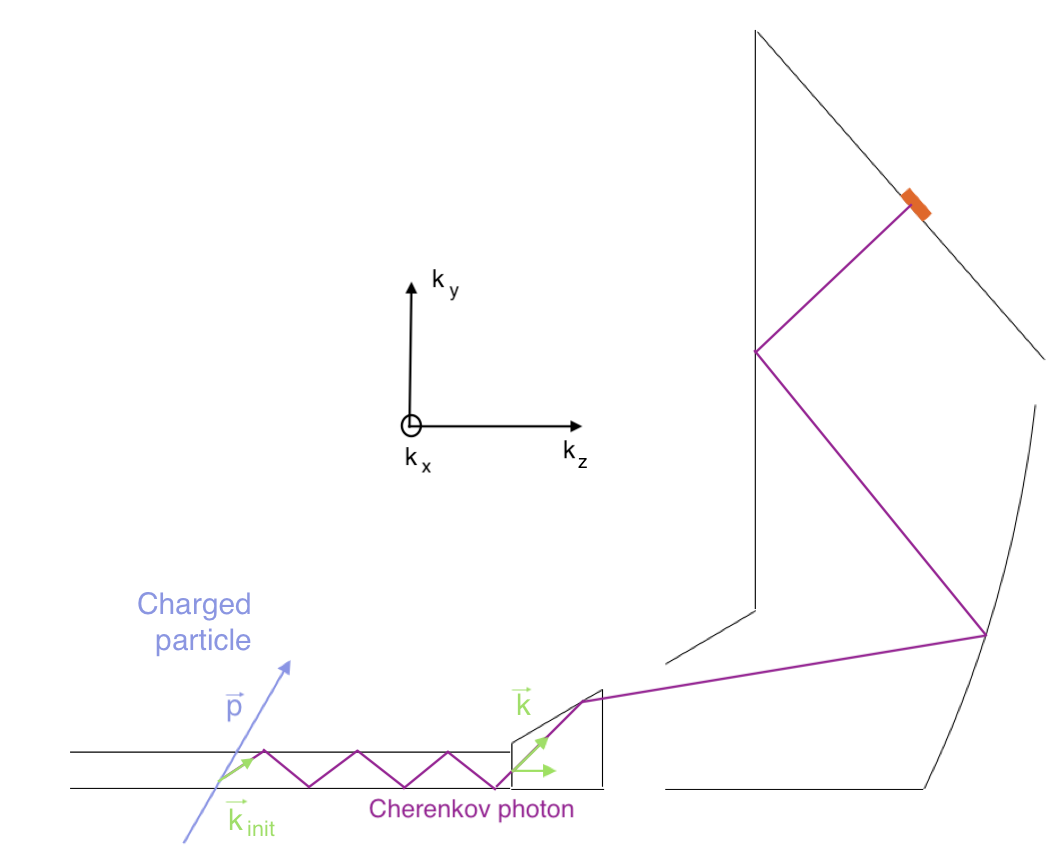
\includegraphics[width=0.6\textwidth]{pics/lut3.png}
\caption{\label{pic:lut1}
The concept of the geometrical reconstruction. One example Cherenkov photon is emitted by the charged particle. The photon direction $\vec k$ is an estimator of the initial photon direction $\vec k_{init}$ and is used to reconstruct $\theta_{C}$ for this photon (using charged particle direction $\vec p$). The photon transportation is described in the bar coordinate system, shown in the insert, which differs from the \gluex coordinate system used so far. In that case a reflection off a particular side results into a sign flip of the corresponding photon direction component.
}
\end{figure}

\begin{figure}[!h]
\centering
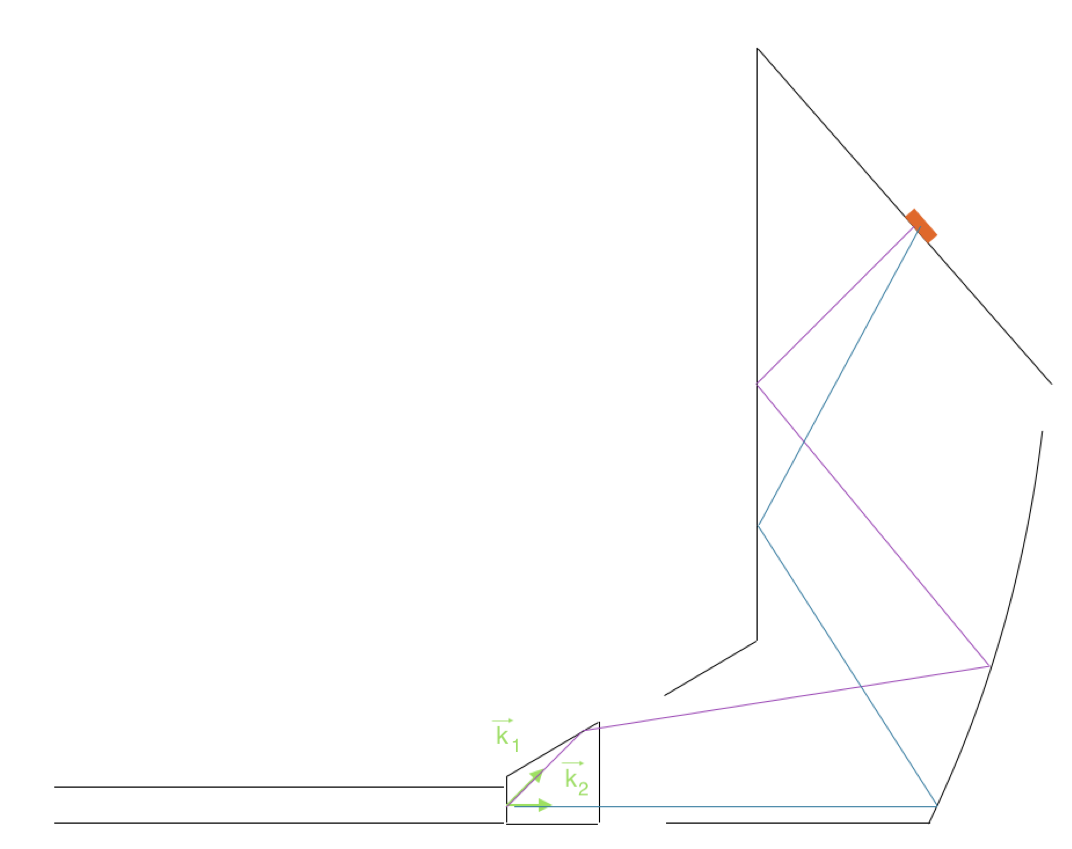
\includegraphics[width=0.6\textwidth]{pics/lut1.png}
\caption{\label{pic:lut2}
An illustration of one entry of the look-up table. Two photons with direction vectors $\vec k_{1}$ and $\vec k_{2}$ originate at the center of the bar, propagate throught the optical box, and end up in the same pixel. The look-up table entry corresponding to the shown pixel contains all possible propagation paths, including $\vec k_{1}$ and $\vec k_{2}$, and the associated propagation times in the small wedge and photon camera.
}
\end{figure}

The reconstruction procedure is the following: each particle crossing the DIRC wall yields a set of hit pixels (e.g. see upper row in Fig.~\ref{pic:hitpat1}). Each detected photon has a set of $N_{pc}$ solutions for the $\vec k$ vectors stored in the LUT. The truth photon direction is then $N_{pc}$ ways ambiguous. Additional reconstruction ambiguities arise from the fact, that the exact photon path during the many internal reflections inside the bar in unknown.  
Each photon direction ambiguity inside the bar corresponds to a reflection off a radiator side. In the bar coordinate system shown in the insert of Fig.~\ref{pic:lut1} a photon reflection off a particular radiator side leads to the sign flip for the corresponding photon direction component. Eight different photon directions are possible inside the bar (including sign flips for forward/backward, top/bottom, and left/right directions). They are taken into account by combining the direction from the LUT in eight different ways with the particle direction, leading to up to eight values for the recontructed photon Cherenkov angle for each $\vec k$ from the LUT entry.
Taking into account both types of ambiguities: $N_{pc}$ inside the photon camera and $8$ inside the radiator bar, for some angles a total number of $50$ and more photon directions is considered in the reconstruction.  This number is reduced by taking into account only photon directions that are internally reflected inside the bar and by requiring the photon Cherenkov angle to be smaller than 1000 mrad ($\approx 57$\mydeg).

%The reconstruction procedure is the following. Each event (a charged particle of some particle type and momentum crosses the DIRC wall) yields a set of hit pixels (e.g. see Fig.~\ref{pic:hitpat1}). Each detected photon has a set of solutions for the $\vec k$ vectors stored in the ''look-up'' table (see Fig.~\ref{pic:lut2}). 
%A three-dimensional photon direction vector $\vec k$ (see Fig.~\ref{pic:lut1}) origins from the center of the bar end and defines the photon path through the optical box ending in the given pixel.  
%Each $\vec k$ vector yields a set of $8$ solutions for the initial photon direction $\vec k_{init}$ (see Fig.~\ref{pic:lut1}), as the photon can effectively be reflected off any side inside the bar (see bar coordinate system depicted in Fig.~\ref{pic:lut1}).
%Together with the track direction, each $\vec k_{init}$ gives one hypothesis for the reconstructed Cherenkov angle of the photon. 

\begin{figure}[!h]
\centering
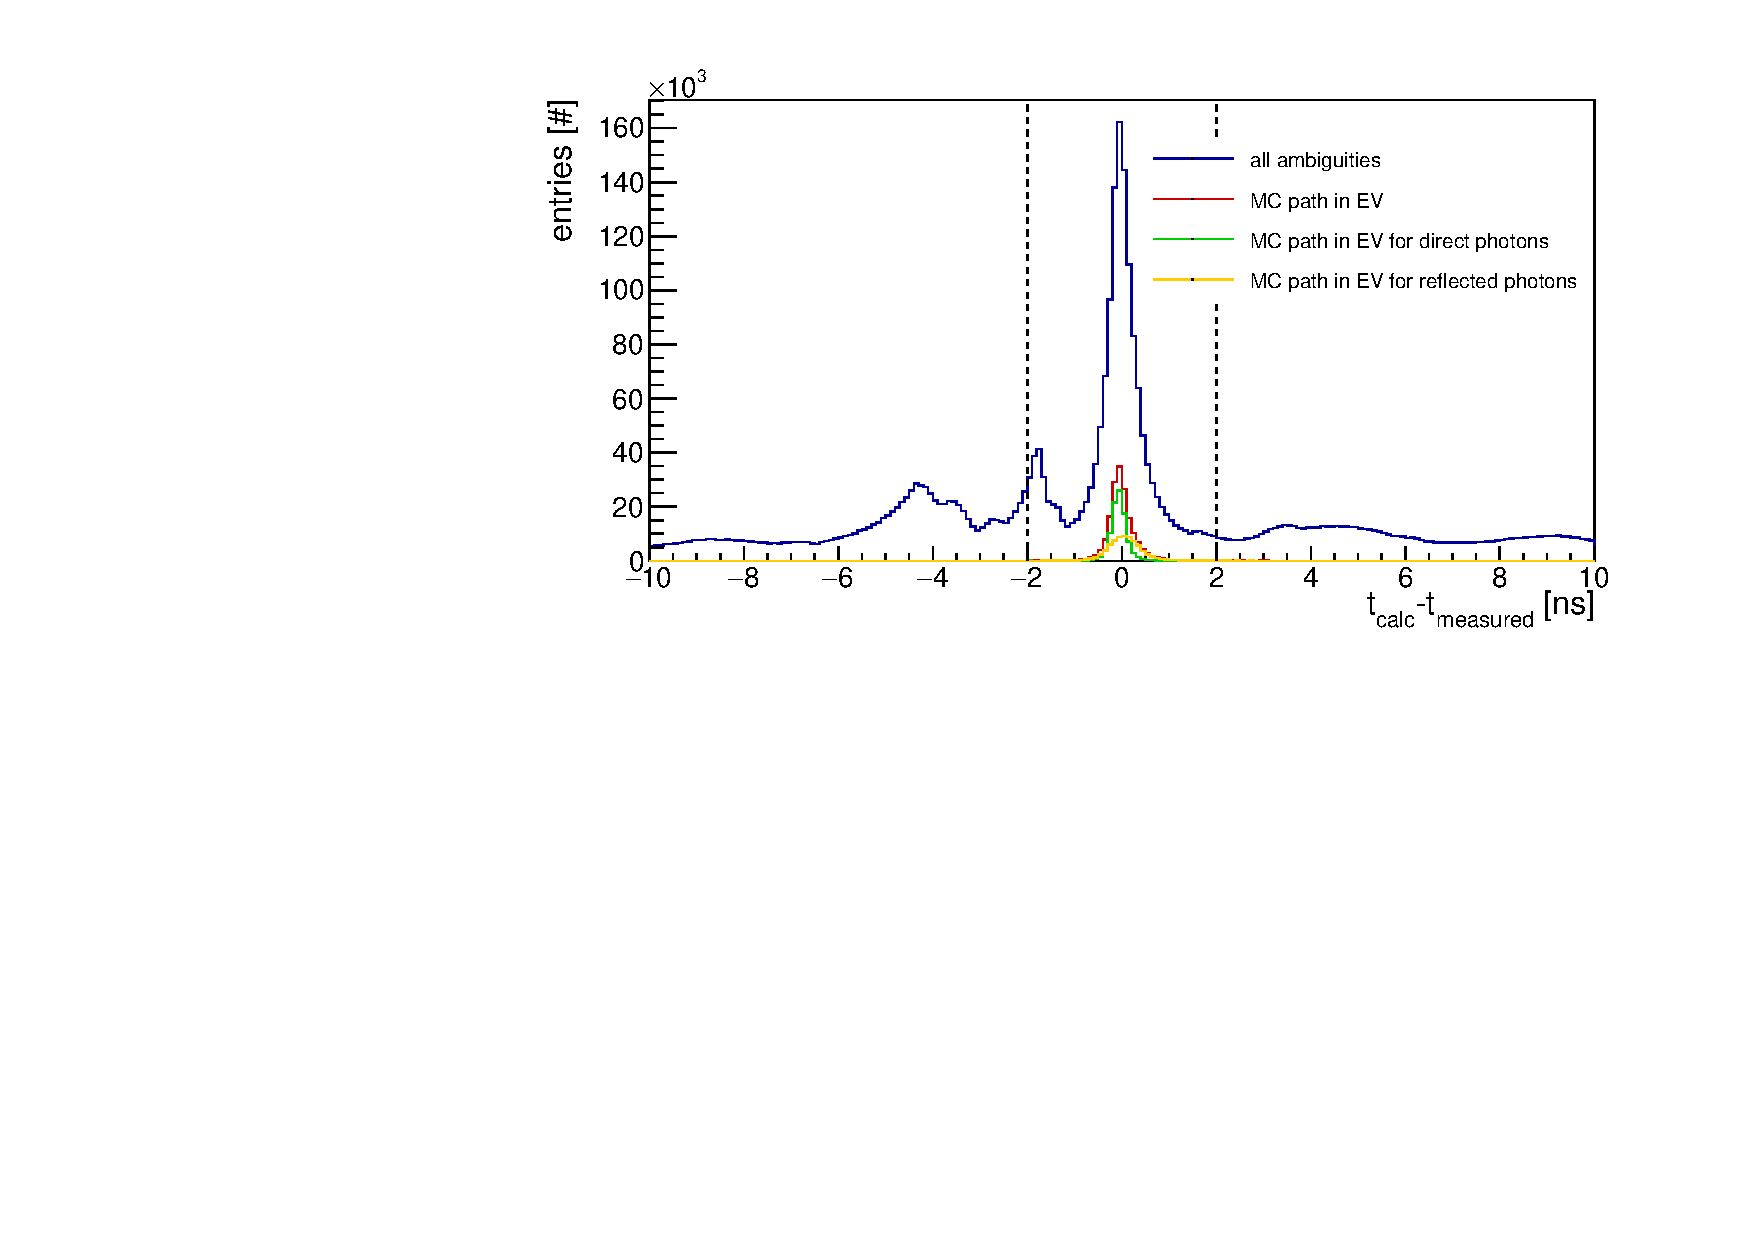
\includegraphics[width=0.8\textwidth]{pics/hDiff.pdf}
\caption{\label{pic:dtime}
Difference between measured and expected arrival time of Cherenkov photons. The blue line shows all solutions including bar and photon camera ambiguities. The red line includes bar ambiguities and a truth photon path inside the photon camera. The green and yellow lines show contributions to the red distribution by direct photons and reflected on the mirror at the radiator end photons respectively. The path length for direct photons is several times shorter than for the reflected photons, therefore the time difference gets less smeared for the green, than for the yellow distribution. The dashed lines show the applied cut for $|\Delta t| < 2$ ns. The plot is for 1000 pions with momentum of 4 \gev/c and direction defined by $\theta = 1$\mydeg and $\phi = 90$\mydeg angles.
}
\end{figure}

Most of the reconstructed photon paths correspond to Cherenkov angles far away from the expected value and form a combinatorial background under the peak associated with the correct photon path. A further reduction of the combinatorial background is achieved by applying a selection cut on the difference between the measured arrival time of the photon and the expected arrival time (see Fig.~\ref{pic:dtime}). The expected arrival time is calculated as a sum of the photon propagation times inside the bar and photon camera. The latter is taken from the LUT. The photon propagation time inside the radiator is calculated based on the photon path, reconstructed using photon direction from the LUT, and the group velocity for photons with average wavelength of $376$ nm (see the energy spectrum of detected photons in Fig.~\ref{pic:lam}). This is the average wavelength determined from the simulation.

\begin{figure}[!h]
\centering
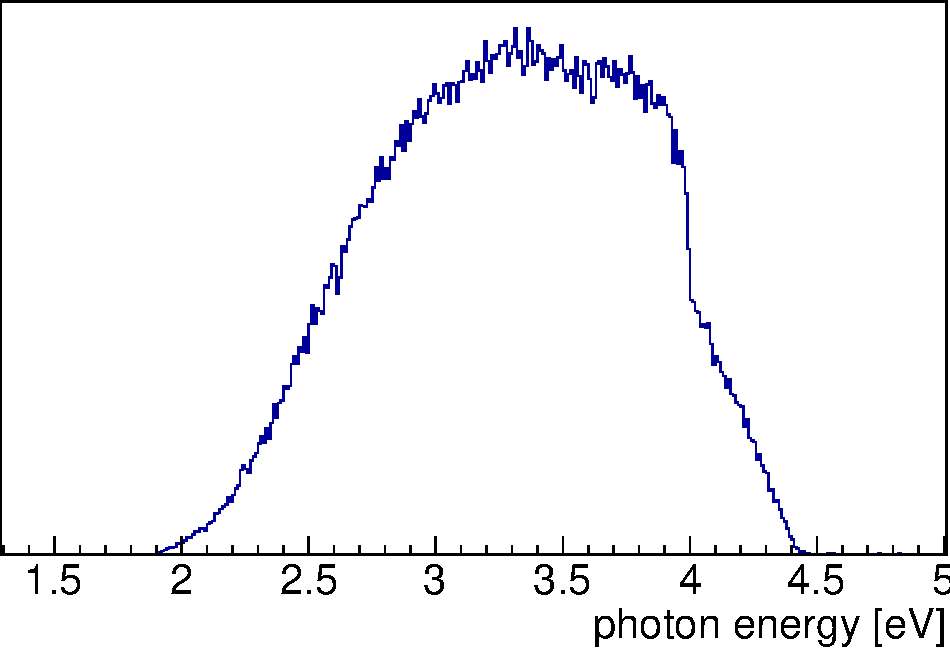
\includegraphics[width=0.4\textwidth]{pics/lam.pdf}
\caption{\label{pic:lam}
Energy spectrum for detected Cherenkov photons. The mean value is $3.3$ eV, which corresponds to $376$ nm.
}
\end{figure}

\begin{figure}[!h]
\centering
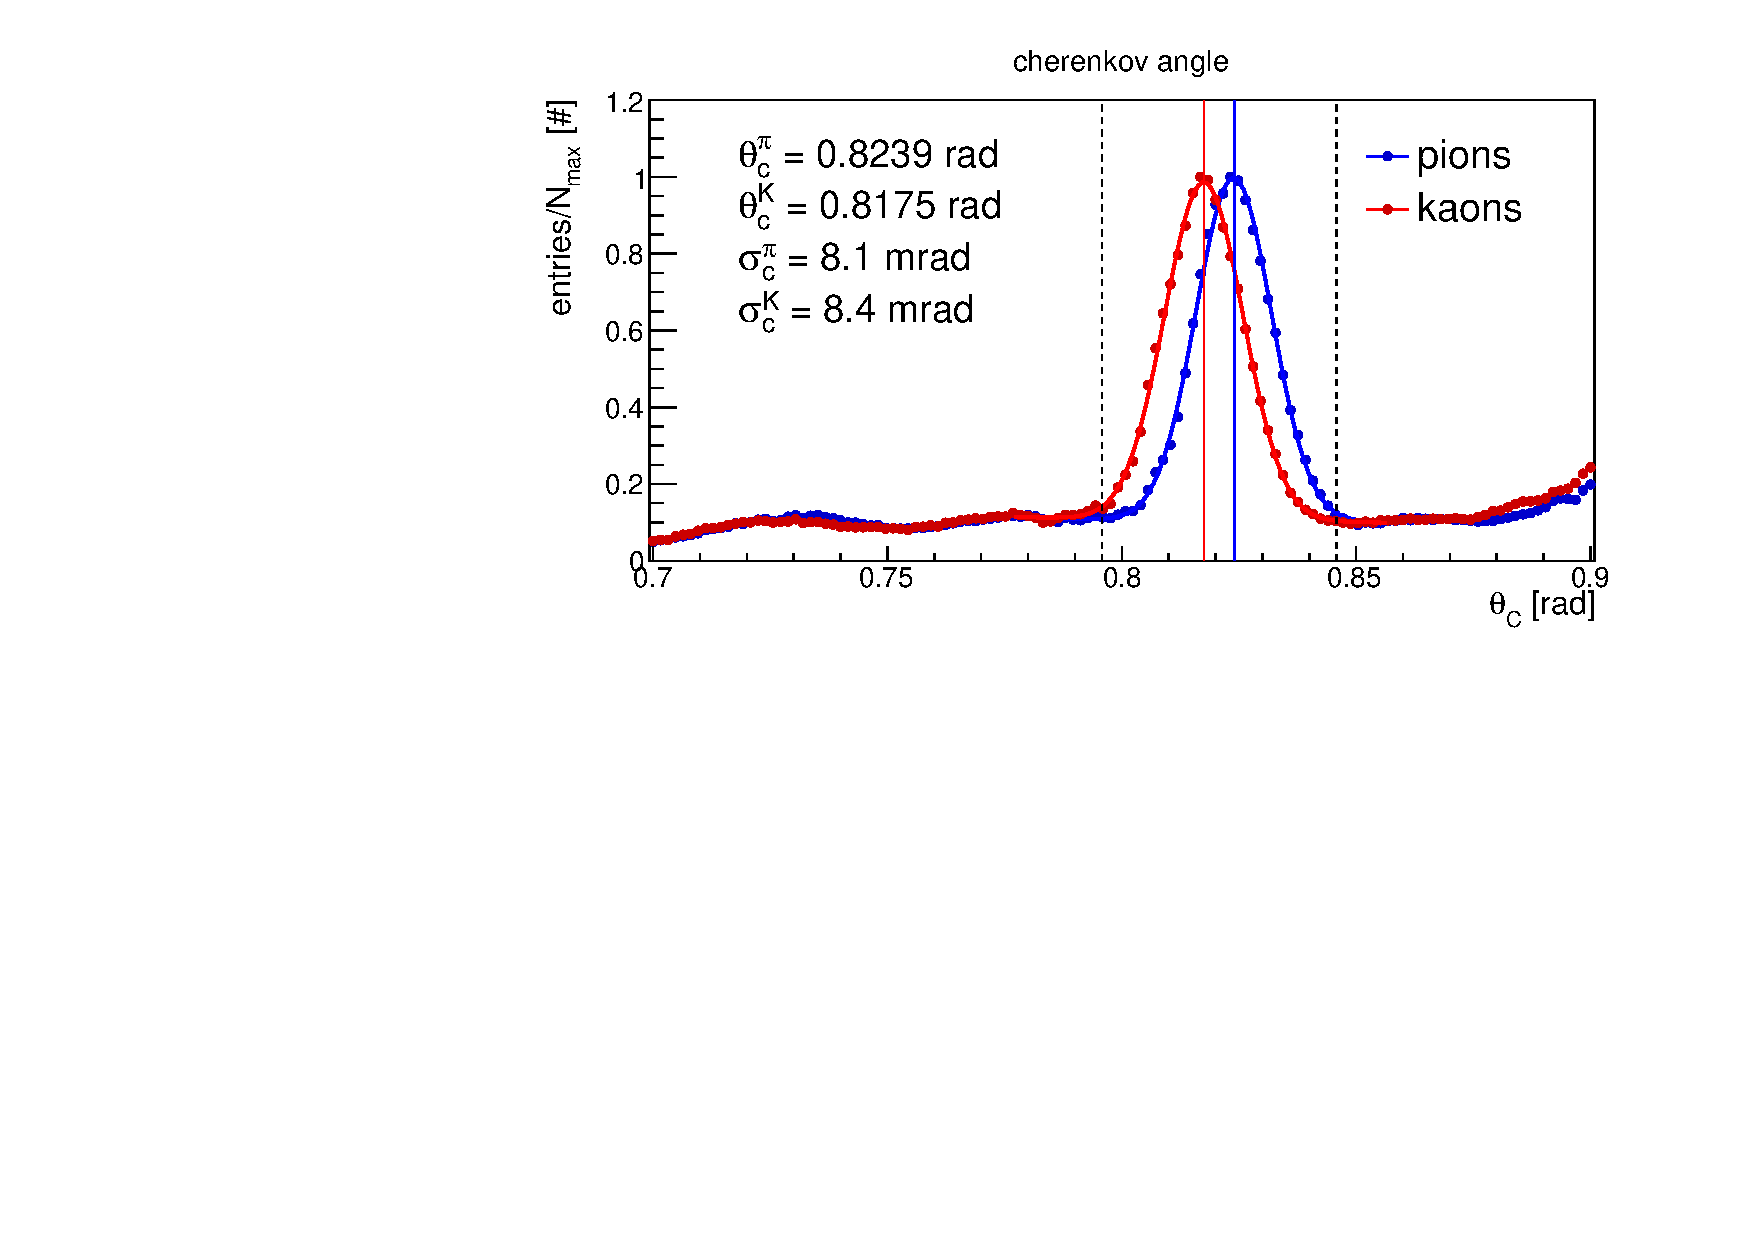
\includegraphics[clip, trim=0cm 0cm 0cm 0.7cm, width=0.8\textwidth]{pics/hAngle.pdf}
\caption{\label{pic:spr}
Cherenkov angles per photon for kaons (red) and pions (blue) with momenta of $4$ {\gev}/c, and direction defined by $\theta = 4$\mydeg and $\phi = 90$\mydeg angles. The solid vertical lines show the expected values for the Cherenkov angles. The dashed lines define the range of values, where the reconstructed photon is considered to be signal (if it also satisfies the cut of time difference). 
%The values of the reconstructed Cherenkov angle and single photon Cherenkov angle resolution are shown.
}
\end{figure}

Going through all the hit pixels for the particle track and collecting the reconstructed Cherenkov angles in a histogram gives a distribution peaking at the expected value of the Cherenkov angle. Figure~\ref{pic:spr} shows the resulting reconstructed Cherenkov angles per photon, including all reconstructed ambiguities, for 1000 pions and kaons with momentum of $4$ {\gev}/c and direction defined by $\theta = 4$\mydeg and $\phi = 90$\mydeg angles. The vertical lines show the expected values for the Cherenkov angle calculated based on the charged particle momentum and the mean refractive index of fused silica. The width of the peak corresponds to the single photon Cherenkov angle resolution $\sigma_{C}$.

An important advantage of the geometrical reconstruction method is that it delivers a measurement of $\sigma_{C}$. Single photon Cherenkov angle resolution is an useful quantity, as it can be measured experimentally and represents the detector resolution, therefore, can be compared to other DIRC and RICH counters. Furthermore, the algorithm is very fast since the LUTs depend only on the detector geometry and not on the particle properties, and thus can be created prior to event resonstruction.

The Cherenkov angle resolution for a track $\sigma_{\theta_{C}}$ can be approximated as the following:

\begin{equation}
\sigma^{2}_{\theta_{C}} = \sigma^{2}_{tr} + \frac{\sigma^{2}_{C}}{N_{\gamma}},
\end{equation}

\noindent where $\sigma_{tr}$ is the tracking resolution, defined by the tracking system (is estimated to be at the order of $1$ mrad~\cite{tdr}), $\sigma_{C}$ -- single photon Cherenkov angle resolution, $N_{\gamma}$ -- number of detected photons per track (based on the simulation it is expected to be between 30 and 60).

There are two ways to perform the PID with the geometric reconstruction. The first way is to extract the reconstructed Cherenkov angle for a charged particle and compare it to the expected values for different hypotheses. The second method is the direct likelihood test.

Log likelihood method of PID compares the measured DIRC signal to the expected signals for different particle hypotheses. In the geometrical reconstruction, each of $N$ hit pixels has a set of $N_{amb}$ Cherenkov angles. The extended log likelihood probability $\log\mathcal{L}$ for a given charged particle hypothesis $h$ ($h = e, \mu, \pi, K, p$) can be defined as~\cite{staric2}:

\begin{equation}
\log\mathcal{L}_{h} = \sum_{i=1}^{N} \sum_{j=1}^{N^{amb}_{i}} \log \Big( S_{h}^{ij} + B_{h}^{ij} \Big) + \log P_{N}(N_{e}),
\label{eq:ll}
\end{equation}

\noindent where $S^{h}_{ij}$ is the signal distribution for the hypothesis $h$, which is the expected value of the Cherenkov angle for the given particle type and momentum, smeared with the measured single photon Cherenkov angle resolution. The distribution is normalized to have the maximum value at $1$. $B^{h}_{ij}$ is the distribution for background (usually described by a linear function). The function $S^{h}_{ij} + B^{h}_{ij}$ for $h = $ kaon and $h = $ pion obtained from the simulation is shown in Fig.~\ref{pic:spr}. $N_{e} = N_{h} + N_{B}$ is the expected number of detected photons, being a sum of the expected number of signal photons $N_{h}$ for hypothesis $h$ and the expected number of background photons, $N_{B}$. The second term in Eq.~\ref{eq:ll} is the Poisson probability to obtain $N$ photons if the mean is $N_{e}$.
%$P_{N}(N)$ is the probability to get the measured number of Cherenkov photons for this hypothesis based on the distribution of the number of expected photons.
During reconstruction, the log likelihood values for the reconstructed Cherenkov photons are summed up for all hit pixels (including all ambiguities). An example of the result is shown in Fig.~\ref{pic:sepLUT}.

\begin{figure}[!h]
\centering
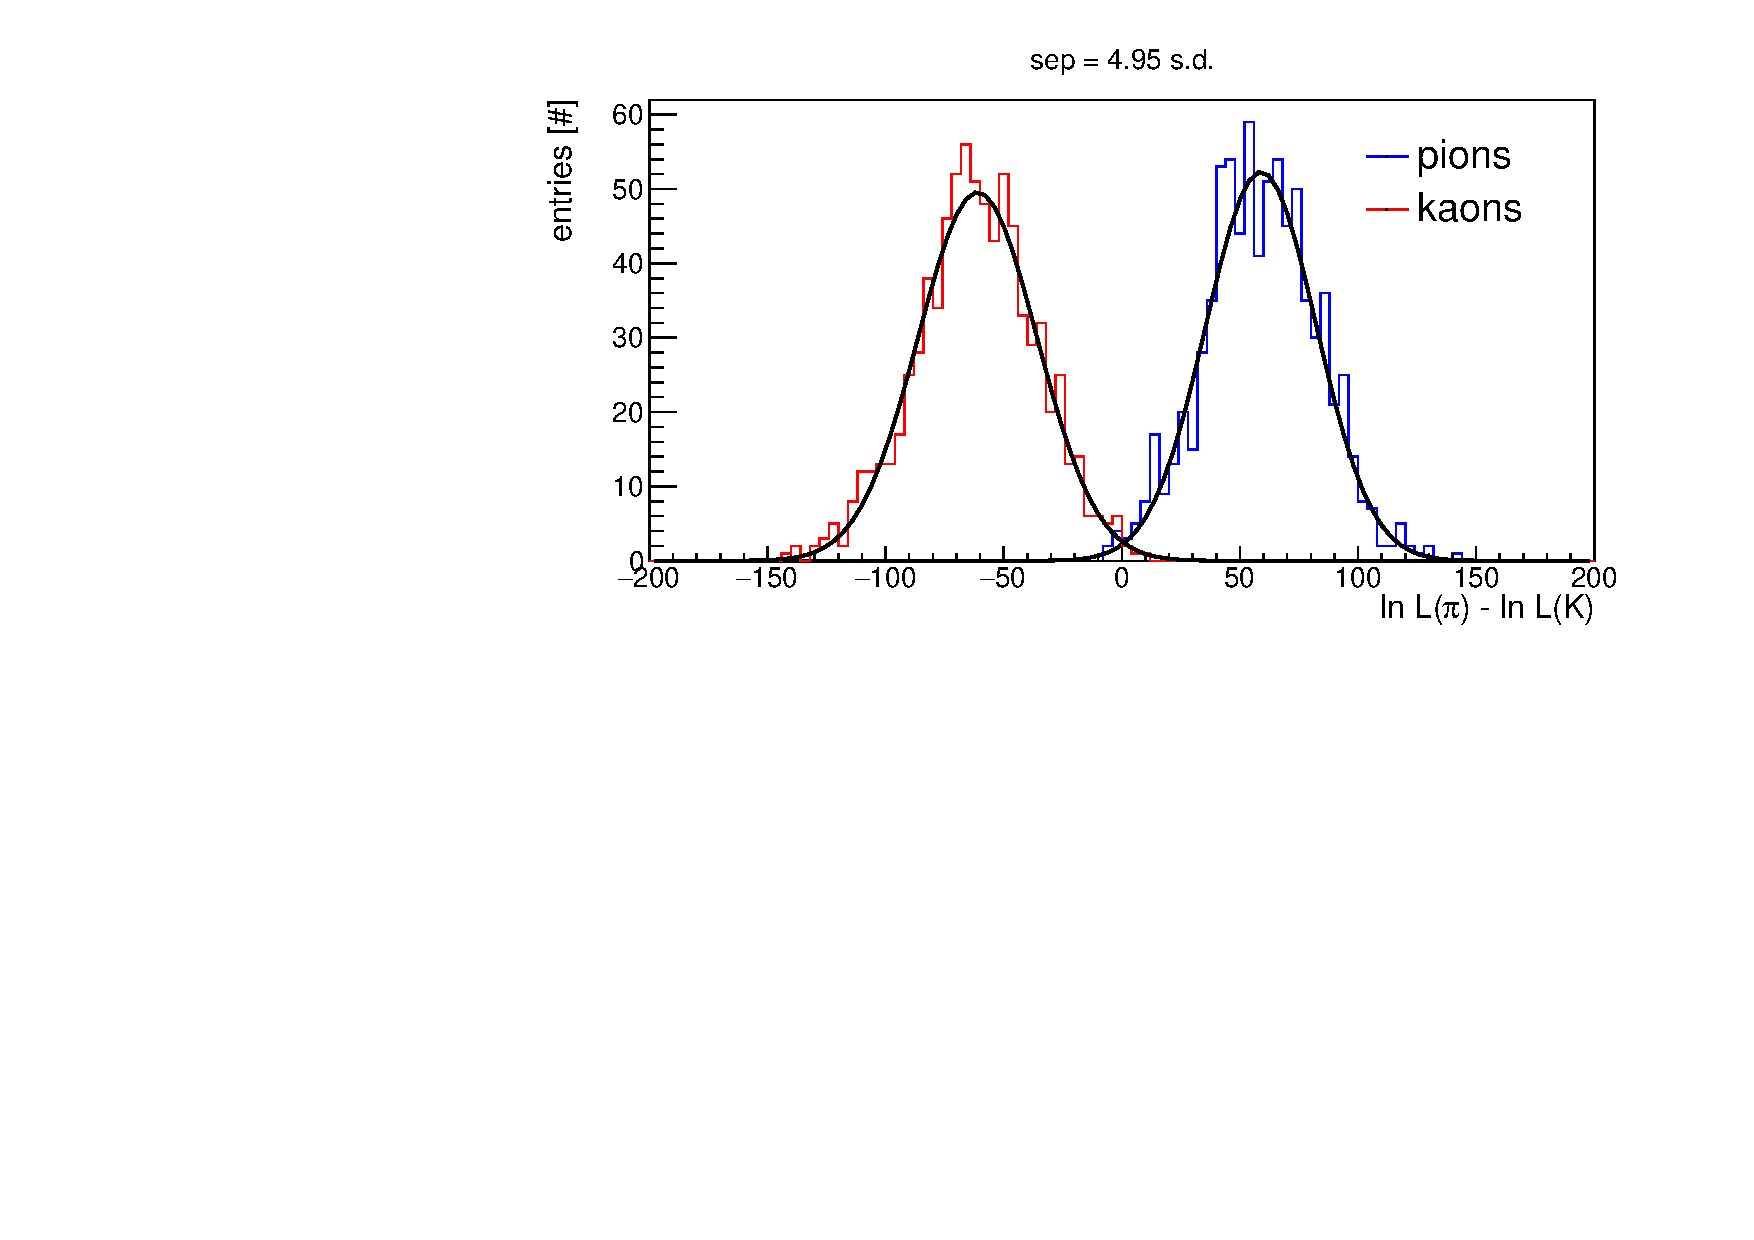
\includegraphics[clip, trim=0cm 0cm 0cm 0.7cm, width=0.8\textwidth]{pics/hLnDiff.pdf}
\caption{\label{pic:sepLUT}
Log likelihood difference (\deltall) between kaons (red) and pions (blue) with momenta of $4$ {\gev}/c, and direction defined by $\theta = 4$\mydeg and $\phi = 90$\mydeg is 4.95 s.d.
}
\end{figure}

The separation $S$ between two hypotheses can be calculated based on the difference in log likelihoods (\deltall):

\begin{equation}
S = \frac{m_{1}-m_{2}}{(\sigma_{1} + \sigma_{2})/2},
\end{equation}

\noindent where $m_{1}$ and $m_{2}$ are the mean values of \deltall for two hypotheses, and the denominator shows the average standard deviation assuming the log likelihood distributions are described by Gauss functions with $\sigma_{1}$ and $\sigma_{2}$.